%! TEX root = ../../main_netxpto.tex
	\subsection{Theoretical Analysis}\label{sec:mqamTeor}
	\subsubsection{QPSK Transmitter}
	\begin{figure}[H]
		\centering
		\centering
		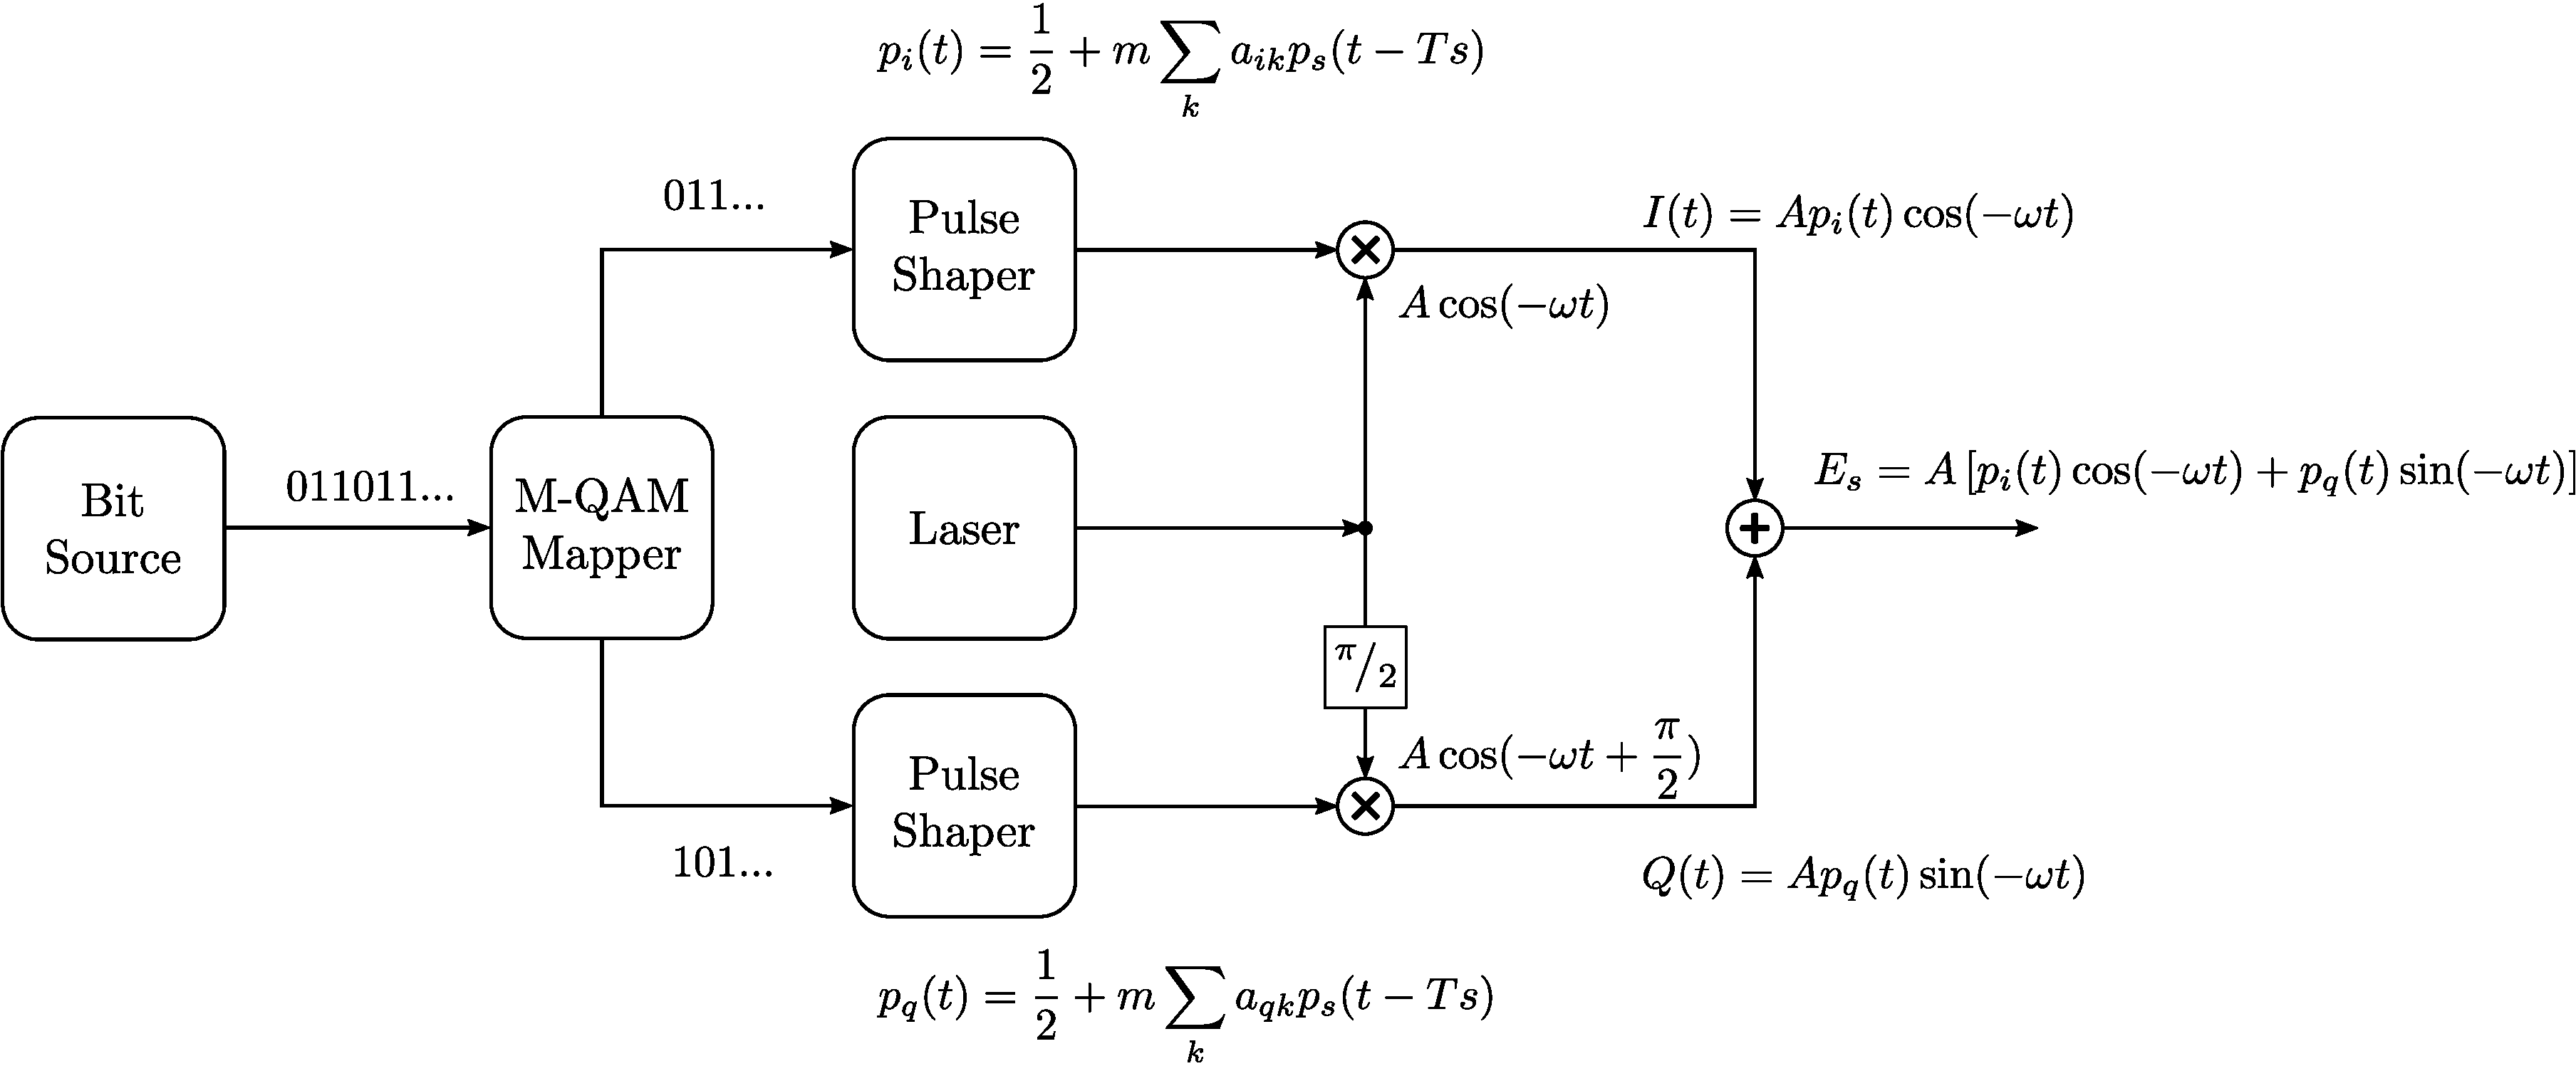
\includegraphics[
		width=0.95\textwidth]{./sdf/m_qam_system/figures/txDiagramTeor.pdf}
		\caption{Transmitter diagram.}
		\label{fig:txDiagramTeor}
	\end{figure}

	M-QAM is a modulation scheme that takes advantage of two sinusoidal carriers
	with a phase difference of $\pi/2$. The resultant output consists of a signal
	with both amplitude and phase variations. For the particular case of M = 4, it
	can be considered that $A_i = A_q = A$ , and therefore $A_c = A \sqrt{2}$.
	The two carriers, referred to as I (In-phase) and Q (Quadrature), can be
	represented as~\cite{carlson86}:

	\begin{align}\label{eq:pulsesi}
		I(t) &= p_i(t) A \cos(-\omega t) \\
		Q(t) &= p_q(t) A \cos\left(-\omega t + \frac{\pi}{2}\right) = p_q(t) A \sin(-\omega
		t) \label{eq:pulsesq}
	\end{align}

	Here, $p_i(t)$ and $p_q(t)$ is the sequence of pulses for each of the
	components, as defined by:

	\begin{equation}\label{eq:pulseDef}
				p(t) = \frac{1}{2}+m \sum_k{a_k p_s(t-T_s)},
				\qquad a_k =
					\begin{cases}
						-1       & \text{if bit} = 1, \\
						1        & \text{if bit} = 0
					\end{cases}
	\end{equation}

	\noindent where m is a scaling coefficient, to ensure the following
	conditions are met

	\begin{equation*}
		\begin{cases}
			\frac{1}{2}+m \left(\max\left\{p_s(t)\right\}\right) = 1 \\
			\frac{1}{2}+m p_s(t) > 0
		\end{cases}
	\end{equation*}

	Following from equations~\ref{eq:pulsesi} and~\ref{eq:pulsesq}, we
	have~\cite{apostol67,oo12}:

	\begin{equation}\label{eq:sigEq}
		\begin{split}
			E_s(t) &= I(t) + Q(t)  = \\
					 &= p_i(t) A\cos(-\omega t)+ p_q(t) A\sin(-\omega t) \\
					 &= p_i(t) A\cos(\omega t)- p_q(t) A\sin(\omega t) \\
					 &= A \sqrt{p_i^2(t) + p_q^2(t)} \cos{\left(- \omega t +
					 \phi_s(t)\right)}, \quad  \phi_s(t)=
					 \operatorname{arctan}{\left({p_q(t)},{p_i(t)}\right)}
		\end{split}
	\end{equation}

	The \textit{arctan} function shown above is the two argument arctangent
	function, sometimes also called \textit{atan2}. While
	the normal arctangent is defined only for the interval~$\left]-\frac{\pi}{2},
	+\frac{\pi}{2}\right]$, the two argument arctangent is a piecewise function
defined in the interval~$\left]-{\pi}, +{\pi}\right]$~\cite{glisson11}.

	\begin{align}
		\arctan(x,y) = \begin{cases}
			\arctan(y/x),                                  & if x > 0,\\
			\left(\operatorname{sign}\left\{y\right\}\right) \left({\pi}/{2}\right)  & if x = 0~\text{and}~y \neq 0, \\
			\pi +  \operatorname{arctan}({y/x})            & if x < 0, \\
			0,                                             & if x = 0~\text{and}~y = 0
		\end{cases}
	\end{align}

%		a(t) = \begin{cases}
%			A               & 0 \le t \le T_s\\
%			0               & t > T_s\\
%		\end{cases}

%	The expression for the electric field when $t_s = n T_s$ becomes:
%
%	\begin{equation}\label{eq:elFieldConst}
%		\begin{split}
%			E_s(t) &= {A} \sqrt{2} \cos{\left[ -\omega t
%					 +\operatorname{arctan}{(p_q(t_s), p_i(t_s))} \right]}\\
%					 &= \frac{A_c}{\sqrt{2}} \sqrt{2} \cos{\left[ -\omega t
%					 +\operatorname{arctan}{(p_q(t_s), p_i(t_s))} \right]}\\
%					 &= A_c \cos{\left( -\omega t + \phi_s(t)\right)}
%%						 \quad \phi_s(t)\in \left[\frac{\pi}{4},\frac{3\pi}{4},\frac{5\pi}{4},\frac{7\pi}{4} \right]
%		\end{split}
%	\end{equation}


	\subsubsection{QPSK Receiver}\label{sec:teorRX}
	We will consider a homodyne receiver with phase diversity. This is a
	configuration which uses a local oscillator with the same optical frequency,
	and measures both the in-phase and the quadrature component at the same time.

	A typical configuration for this receiver is shown in
	Figure~\ref{fig:rxDiagram}. The local oscillator laser uses the same frequency
	of the incoming signal. It is used in coherent
	detection to extract the phase and amplitude information contained in the received optical
	signal. This is done by mixing the LO with the incoming optical signal in a
	${\pi}/{2}$ optical hybrid. The optical hybrid then outputs 4 different
	optical signals, where the phase difference between the LO and the signal is
	at $0$, ${\pi}/{2}$, ${\pi}$, ${3\pi}/{2}$. This difference is relative to
	their phase difference at the input of the optical hybrid. The signals with a
	difference of $\pi$ between themselves are paired and sent to a pair of
	balanced photodiodes, where each pair measures one of the quadratures. The
	transimpedance amplifier then amplifies the signal, while converting the
	current to a voltage to be sampled and quantified in an ADC.



	\begin{figure}[H]
		\centering
		\centering
		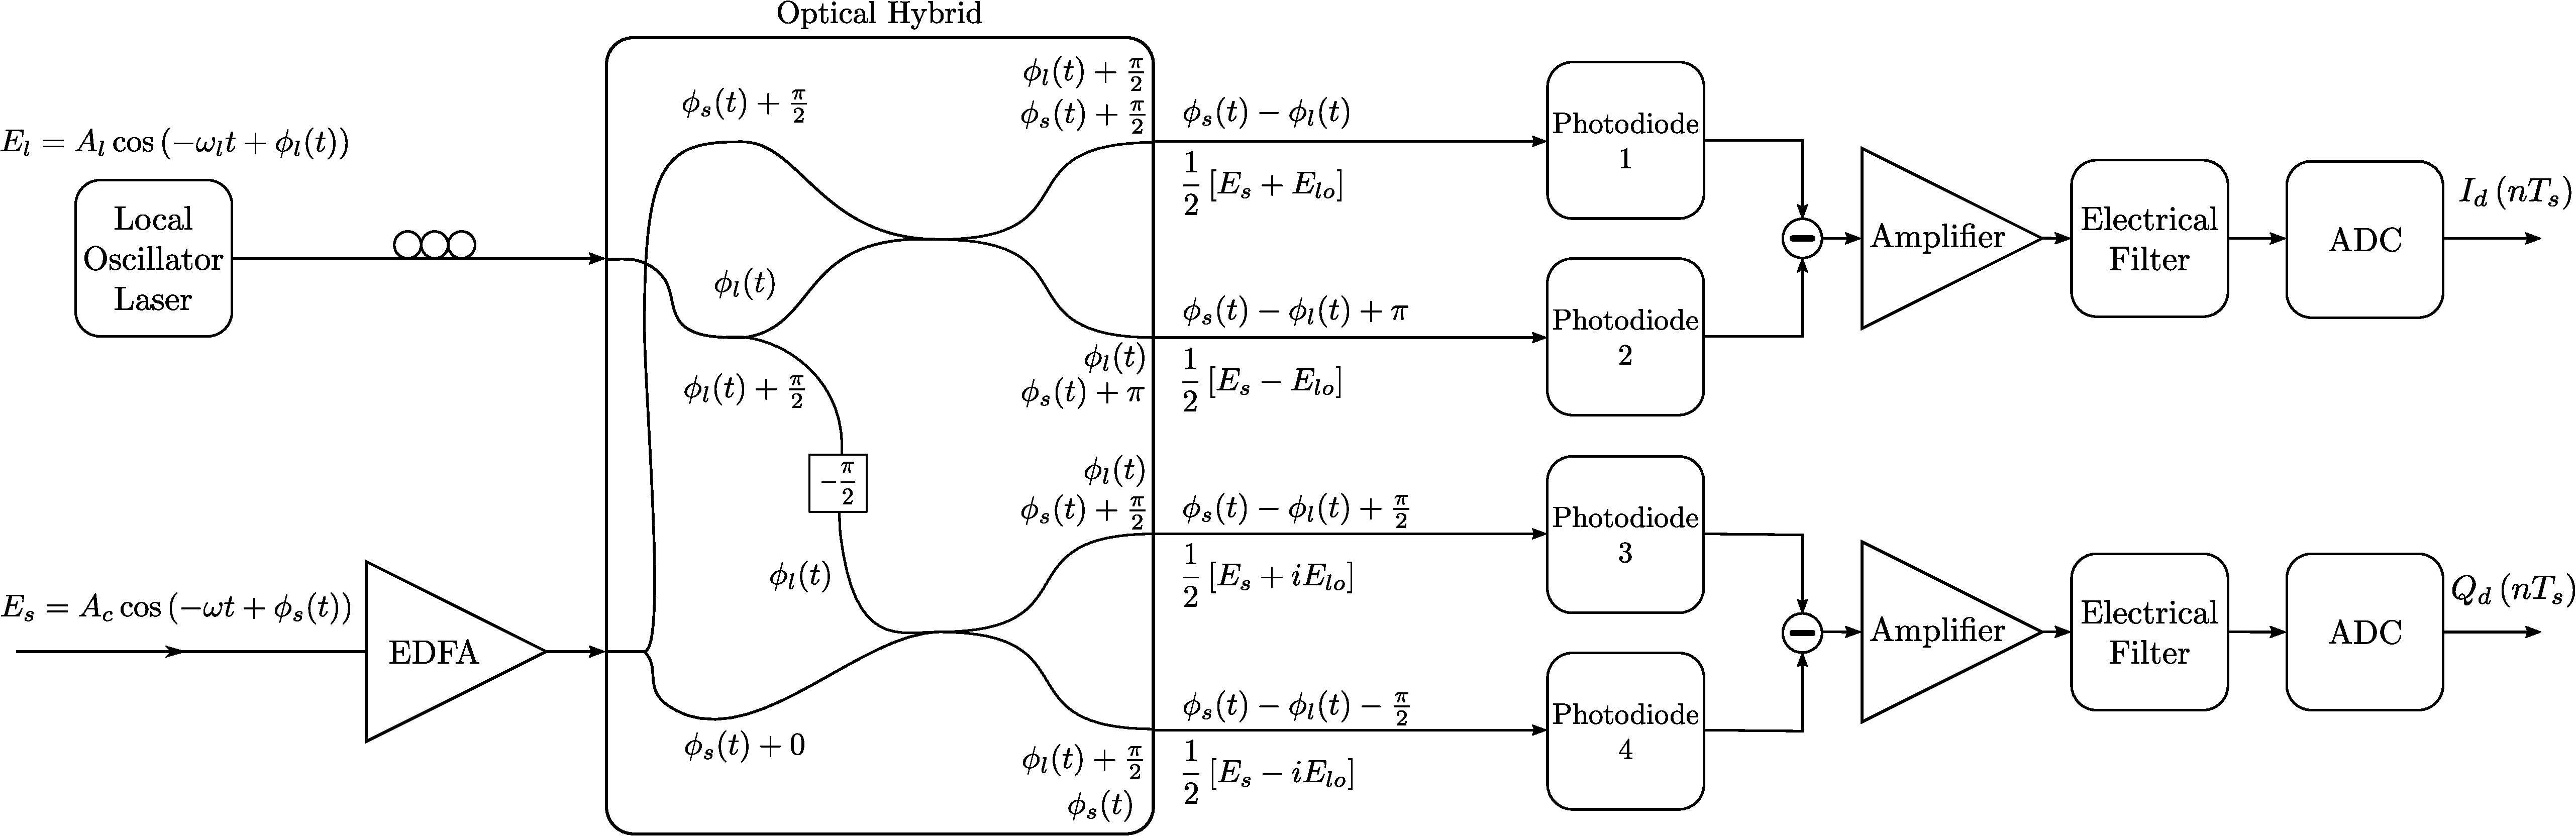
\includegraphics[width=0.95\textwidth]{./sdf/m_qam_system/figures/rxDiagramTeor_edfa.pdf}
		\caption{\label{fig:rxDiagram} Local oscillator and receiver filters
		diagram. $\phi_a$ and $\phi_b$ represent the phase rotations happening
	inside the optical hybrid.}
	\end{figure}

	Before starting, we should clarify how the optical hybrid works. A possible
	configuration is shown in Figure~\ref{fig:rxDiagram}, where the mixing is
	achieved resorting to a few directional couplers. Figure~\ref{fig:coupler}
	shows an example of a directional coupler, where two fiber cores are close enough so that the space
	between them is comparable to their diameter. In these conditions, the
	fundamental modes propagating through each fiber overlap partially, leading to
	power transfer from one core to the other~\cite{agrawal04}.

	\begin{figure}[H]
		\centering
		\centering
		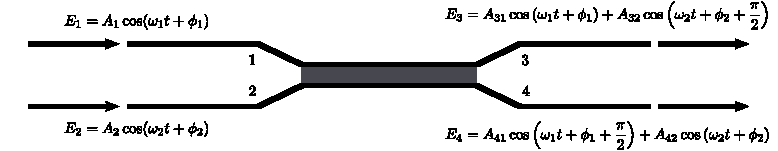
\includegraphics[width=0.95\textwidth]{./sdf/m_qam_system/figures/coupler.pdf}
		\caption{\label{fig:coupler} Directional coupler diagram.}
	\end{figure}

%	Consider the ratio between output and input power to be given by $\rho =
%	P_{o}/P_{i}$. The transfer matrix of a coupler following that relation is:
%
	Assuming a lossless directional coupler as shown Figure~\ref{fig:coupler},
	the relation between input and output power is:

	\begin{equation}\label{eq:couplerPower}
		P_1 + P_2 = P_3 + P_4
	\end{equation}


	With this in mind, the amplitudes $A_3$ and $A_4$
	on the output of a coupler are related to their inputs $A_1$ and $A_2$ by the
	coupling length $L$ and the coupling coefficient $k$:

	\begin{equation}\label{eq:couplerInOut}
	\begin{bmatrix}
		A_3 \\
		A_4 \\
	\end{bmatrix}
	=
	\begin{bmatrix}
		\cos(kL) & i\sin(kL) \\
		i\sin(kL) & cos(kL) \\
	\end{bmatrix}
	\begin{bmatrix}
		A_1 \\
		A_2 \\
	\end{bmatrix}
\end{equation}
% Considering an input on port 1, indicated on the diagram as $E_1$, the relation
% between the power at that point and at ports 3 and 4 is:
%
% \begin{align}
%	 P_3 (L_c) &= P_1 \cos^2(k_cL_c) \\
%	 P_4 (L_c) &= P_1 \sin^2(k_cL_c)
% \end{align}

Two things can be noticed here: first, the power ratios are dependent on the coupling
 length. This comes from the supermodes of the fiber coupler, which have
 different propagation constants~\cite{agrawal04}. This difference creates a relative phase shift
 proportional to the coupler length. In addition, a phase shift of $\pi/2$
 exists always between the two outputs. This is because the supermodes are the
 even and odd combinations of the fundamental modes of the coupler.

 This phase shift can be taken advantage of to create an optical hybrid, by mixing
 the components in a way to end up with 4 different combinations of the signal
 and LO, having relative phase differences of $0, \pi/2, \pi$ and $3\pi/2$.

% The power dependece comes from the supermodes of the fiber coupler, which have
% different propagation constants. Assuming the coupler to be symmetric, the
% modes are the even and odd combinations of the fundamental modes.
%
% both modes excited, a relative phase difference exists due to the different
% propagation constants of the modes. In addition, as the fi



%	Consider the ratio between output and input power to be given by $\rho =
%	P_{o}/P_{i}$. The transfer matrix of a coupler following that relation is:
%
%	The amplitudes $A_3$ and $A_4$ on the output of a coupler are related to their
%	inputs A_1 and A_2 by the coupling length L and the coupling coefficient k:
%
%	\begin{equation}
%	\begin{bmatrix}
%		A_3 \\
%		A_4 \\
%	\end{bmatrix}
%	=
%	\begin{bmatrix}
%		\cos(kL) & i\sin(kL) \\
%		i\sin(kL) & cos(KL) \\
%	\end{bmatrix}
%	\begin{bmatrix}
%		A_1 \\
%		A_2 \\
%	\end{bmatrix}
%\end{equation}

	We can now proceed to analyze the process at the receiver, but for now we will
	ignore the noise added by the EDFA shown at the beginning of the
	diagram.

	Coherent detection takes the product of the electric fields from the signal and
	a Local Oscillator, in order to measure the phase difference between them
	through interference. The electric field of the Local Oscillator
	is~\cite{kikuchi16}:

	\begin{equation}
		%E_{lo} = A_{lo} e^{i(-\omega_{lo} t + \phi_{lo})}
		E_{lo} = A_{lo} \cos{(-\omega_{lo} t + \phi_{lo})}
	\end{equation}

	The amplitudes $A_{lo}$ and $A_c$ are related to their respective average optical power by:

	\begin{align*}
		P_s    &= k {E_s}^2    = k {A_c}^2 \cos^2(-\omega t + \phi_s) = k
		\frac{{A_c}^2}{2} = k \frac{{(A \sqrt{2})}^2}{2} = k A^2 \\
		P_{lo} &= k {E_{lo}}^2 = k {A_{lo}}^2 \cos^2(-\omega_{lo} t + \phi_{lo}) = k \frac{{A_{lo}}^2}{2}
	\end{align*}

	\noindent where $k$ is the ratio between the effective beam area and the impedance of free
	space. The power of the signal entering the EDFA is amplified by a gain factor $G_o$

	\begin{equation}
		P_{\text{s\_out}} = G_o P_{\text{s\_in}}
	\end{equation}

	\noindent	$G_o$ is the EDFA optical gain, given by~\cite{mukai81}:

	\begin{equation}\label{fig:ampGain}
		G_o = \frac{G_\text{small}}{1+\frac{P_\text{in}}{P_{\text{sat}}}}
	\end{equation}

	\noindent where $G_\text{small}$ is the gain for small signals, $P_\text{in}$ is
	the optical power at the EDFA's input and $P_\text{sat}$ is the EDFA's
	saturation power. This means that the effective optical gain is lower for
	input signals with higher optical powers.


	As the input optical signal and local oscillator enter the optical hybrid,
	each of them is split twice in 3-dB couplers. This means that a quarter of the
	power from each source reaches each of the photodiodes. In addition, as
	previously explained, they are subject to phase shifts which mix them with
	differente relative phase differences.
	We therefore get 4 different combinations from $E_s$ and$E_{lo}$, the
	electrical fields of the signal and the LO.

	\begin{align*}
		E_1 &= \frac{1}{2}\left(\sqrt{G_o} E_s + E_{lo}\right) \\
		E_2 &= \frac{1}{2}\left(\sqrt{G_o} E_s - E_{lo}\right) \\
		E_3 &= \frac{1}{2}\left(\sqrt{G_o} E_s + i E_{lo}\right) \\
		E_4 &= \frac{1}{2}\left(\sqrt{G_o} E_s - i E_{lo}\right) \\
	\end{align*}

	Let us assume from now on that $\omega = \omega_{lo}$ and $\phi_{lo} = 0$. In
	this case, the photocurrent for the each of the previous n combinations is
	equal to:

%	\begin{align}
%		I_1 (t) &= \frac{R}{4} \left[ P_s(t) + P_{lo} + 2 \sqrt{P_s(t)P_{lo}}
%						\cos{(\phi_s(t) - \phi_{lo}(t))}\right] \\
%		I_2 (t) &= \frac{R}{4} \left[ P_s(t) + P_{lo} - 2 \sqrt{P_s(t)P_{lo}}
%						\cos{(\phi_s(t) - \phi_{lo}(t))}\right] \\
%		I_3 (t) &= \frac{R}{4} \left[ P_s(t) + P_{lo} + 2 \sqrt{P_s(t)P_{lo}}
%						\sin{(\phi_s(t) - \phi_{lo}(t))}\right] \\
%		I_4 (t) &= \frac{R}{4} \left[ P_s(t) + P_{lo} - 2 \sqrt{P_s(t)P_{lo}}
%						\sin{(\phi_s(t) - \phi_{lo}(t))}\right] \\
%	\end{align}

	\begin{align}
		I_1 (t) &= \frac{\eta}{4} \left[ G_o P_s(t) + P_{lo} + 2 \sqrt{G_o P_s(t)P_{lo}}
						\cos{\big(\phi_s(t)\big)}\right] \\
		I_2 (t) &= \frac{\eta}{4} \left[ G_o P_s(t) + P_{lo} - 2 \sqrt{G_o P_s(t)P_{lo}}
						\cos{\big(\phi_s(t)\big)}\right] \\
		I_3 (t) &= \frac{\eta}{4} \left[ G_o P_s(t) + P_{lo} + 2 \sqrt{G_o P_s(t)P_{lo}}
						\sin{\big(\phi_s(t)\big)}\right] \\
		I_4 (t) &= \frac{\eta}{4} \left[ G_o P_s(t) + P_{lo} - 2 \sqrt{G_o P_s(t)P_{lo}}
						\sin{\big(\phi_s(t)\big)}\right] \\
	\end{align}

	\noindent where $\eta$ is the photodiodes' responsivity.
	Two photocurrents are generated from the combination of the balanced photodiodes,
	which are then amplified in a transimpedance amplifier with a gain factor $G_e$.

	\begin{align}
		V_i(t) &= G_e\left(I_{1} - I_{2}\right) \notag\\
					 &= G_e \eta \sqrt{G_o P_s P_{lo}} \cos{(\phi_{s}(t))} \label{eq:photocurrentI} \\
		V_q(t) &= G_e\left(I_{3} - I_{4}\right) \notag\\
					 &= G_e \eta \sqrt{G_o P_s P_{lo}} \sin{(\phi_{s}(t))}\label{eq:photocurrentQ}
	\end{align}

	These voltages effectively reconstruct the transmitted optical signal.
	After going through the electrical filter, they can be sampled
	into the digital domain for processing.

	Assuming perfect synchronization, if the signal is sampled with timing $t =
	n T_s$, the constellation can be reconstituted perfectly, if there is no
	intersymbol interference. In this case, according to
	equations~\ref{eq:pulsesi} and~\ref{eq:pulsesq}, $p_i(t)$ and $p_q(t)$ are
	equal to either $1$ or $-1$. It follows that $\phi_s(t = nT_s) = \frac{\pi}{4}
	\pm m \frac{\pi}{2}$. If the gain $G_e$ is adjusted so that $ G_e\eta\sqrt{G_o P_s
	P_{lo}} = A_c$, we get:

	\begin{align}
		V_i(t) &= {A_c} \cos{(\phi_{s}(t))}, \notag \\
					 &= \pm \frac{A_c}{\sqrt{2}} = \pm A_i = \pm A \qquad t = nTs \label{eq:rxSymbolsi} \\
		V_q(t) &= {A_c} \sin{(\phi_{s}(t))}, \notag \\
					 &= \pm \frac{A_c}{\sqrt{2}} = \pm A_q = \pm A \qquad t = nTs \label{eq:rxSymbolsq}
	\end{align}


%	\begin{equation}
%		\begin{split}
%			I (t) &= I_i(t) + I_q(t) \\
%						&= G R \sqrt{P_s P_{lo}}
%		\left[\cos{(\phi_s(t))}+\sin{(\phi_s(t))}\right] \\
%						& = \frac{A_c}{\sqrt{2}}
%		\left[\cos{(\phi_s(t))}+\sin{(\phi_s(t))}\right]
%		\end{split}
%	\end{equation}


	Looking at Figure~\ref{fig:rxConst}, we can see that
	equations~\ref{eq:rxSymbolsi} and~\ref{eq:rxSymbolsq} describe the four points in the
	constellation.

	\begin{figure}[H]
		\centering
		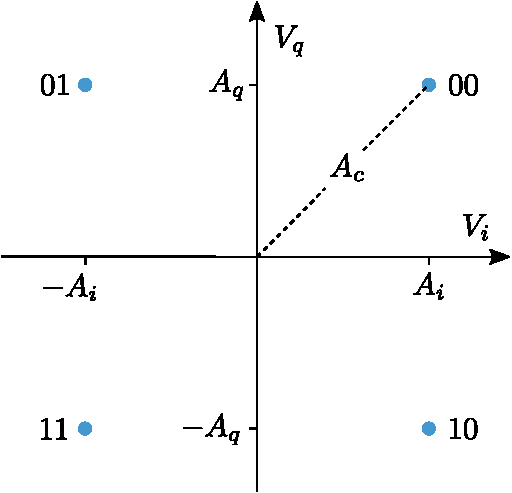
\includegraphics[width=0.5\textwidth]{./sdf/m_qam_system/figures/constellationRx.pdf}
		\caption{A QPSK constellation, assuming $ A = A_i = A_q =
			A_c/\sqrt{2}$.\label{fig:rxConst}}
	\end{figure}

	The previous explanation assumes that the polarization of both the transmitted
	signal and the local oscillator is aligned. This can be achieved by using a
	polarization controller, as shown in Figure~\ref{fig:rxDiagram}. We have also
	neglected any link losses.

	\subsubsection{ISI}\label{sec:ISI}
	We have assumed the absence of intersymbol interference.
	As previously mentioned, bits are coded into the symbols of a given constellation.
	These symbols, associated with a given discrete amplitude, need to be
	encoded into the I and Q carriers. For this, a given shape must be used to
	translate the discrete symbols into continuous, finite pulses in the analog domain.
	The choice of the shape to be used is particularly important for the ISI.

	\begin{figure}[b]
		\centering
		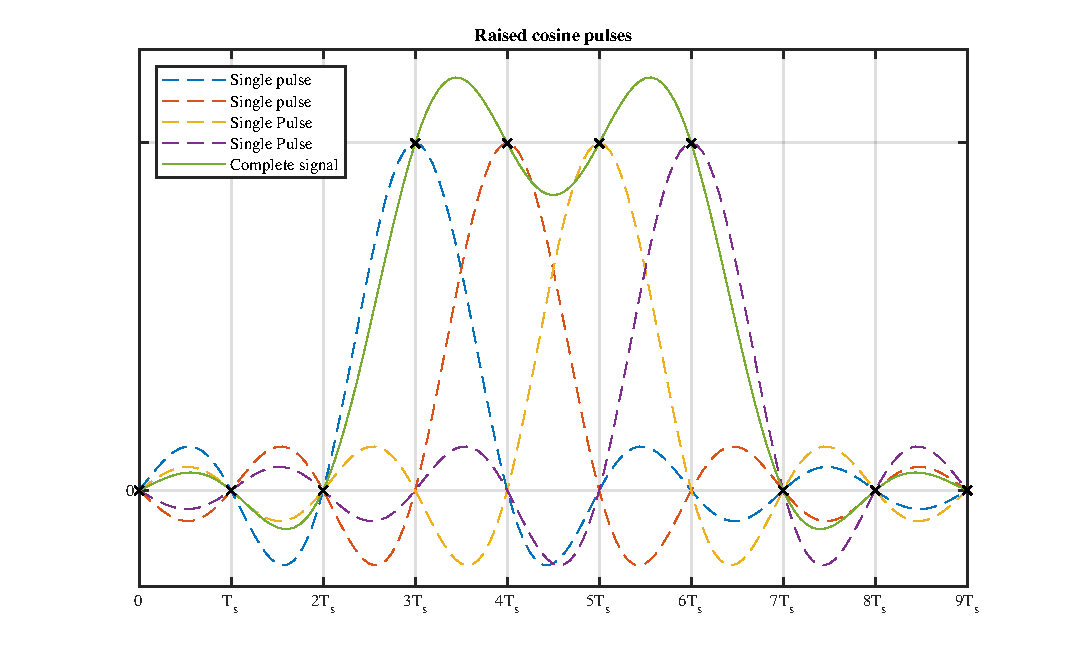
\includegraphics[width=\textwidth]{./sdf/m_qam_system/figures/eyes/ISI/signalAndPulsesRaisedCosine.pdf}
		\caption{Signal generated by four sequential raised cosine pulses. It can be seen
		that at $t=nT_s$, every pulse except one equals exactly zeros, showing that
	there is no interference. In addition, at those times, the value of the signal
is coincident with the peak of the individual pulses.}
\label{fig:ISIRCsig}
	\end{figure}

	Each symbol is represented by its own pulse, which is dependent on the symbol
	period $T_s$. In each pulse, there is an optimal instant $t_s$, where we can sample the signal in
	order to perfectly identify the contained symbol. These instants are separated by a time
	equal to the symbol period. In order to negate intersymbol interference, the
	signal for each pulse should be equal to zero every time a different symbol is
	sampled, that is, at all instants $t_s \pm nT_s$. If this condition is verified,
	the value of the signal at $t=t_s$ is dependent only on the symbol transmitted
	at that time, not being influenced by the surrounding pulses. This is shown in
	Figure~\ref{fig:ISIcomp}, where we can see that at all instants $nT_s$, the
	reponse is zero for all pulses but one. Consequently, at those instants, the
	signal obtained from the combination of all pulses is exactly equal to the peak
	of the pulse transmitted at that time. Those instants are also shown at the
	center of the eye diagram shown in Figure~\ref{fig:ISIcomp}, where $t_s$ is
	represented, and perfect coincidence in the signal at sampling time is shown.

	The raised-cosine is a shape commonly used for pulse shaping, as it does not
	create any intersymbol interference. This is shown in
	Figure~\ref{fig:ISIcomp}. The time domain response for raised-cosine filter is
	given by~\cite{nguyen09}

	\begin{equation} \label{eq:rcTD}
		h_{RC}(t) = \frac{\sin(\pi t/ T_s)}{(\pi t/ T_s)} \frac{\cos(\pi \beta t
		/T_s)}{1-(4\beta^2 t^2/T_s^2)}
	\end{equation}

	\noindent where $\beta$ is the roll-off factor and $T_s$ is the symbol period.

	\begin{figure}
		\centering
		\begin{minipage}{0.45\textwidth}
			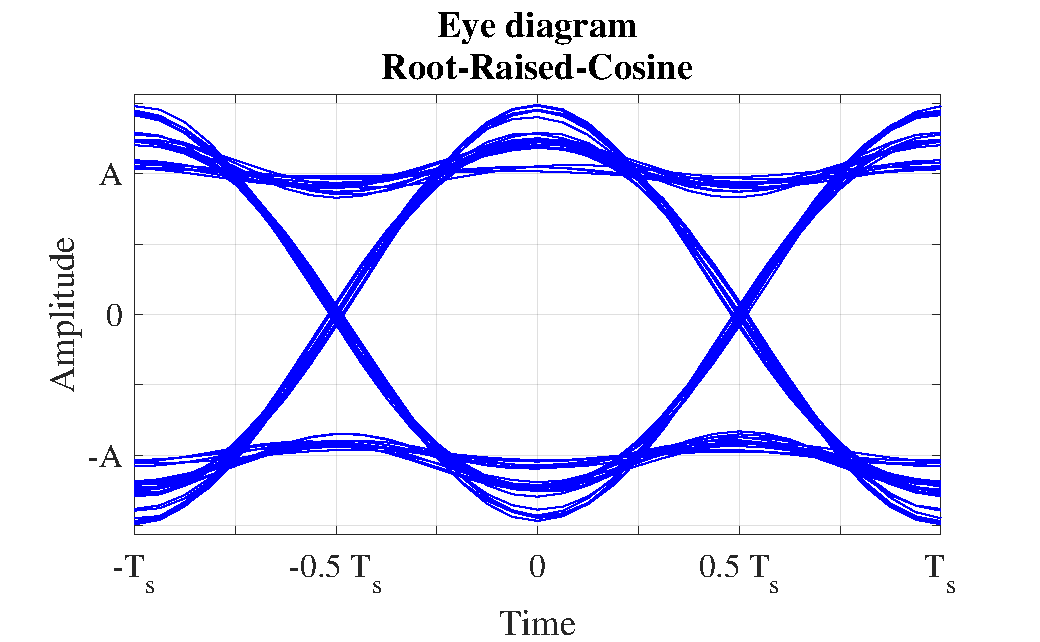
\includegraphics[width=\textwidth]{./sdf/m_qam_system/figures/eyes/ISI/RRC.pdf}
		\end{minipage}
		\begin{minipage}{0.45\textwidth}
			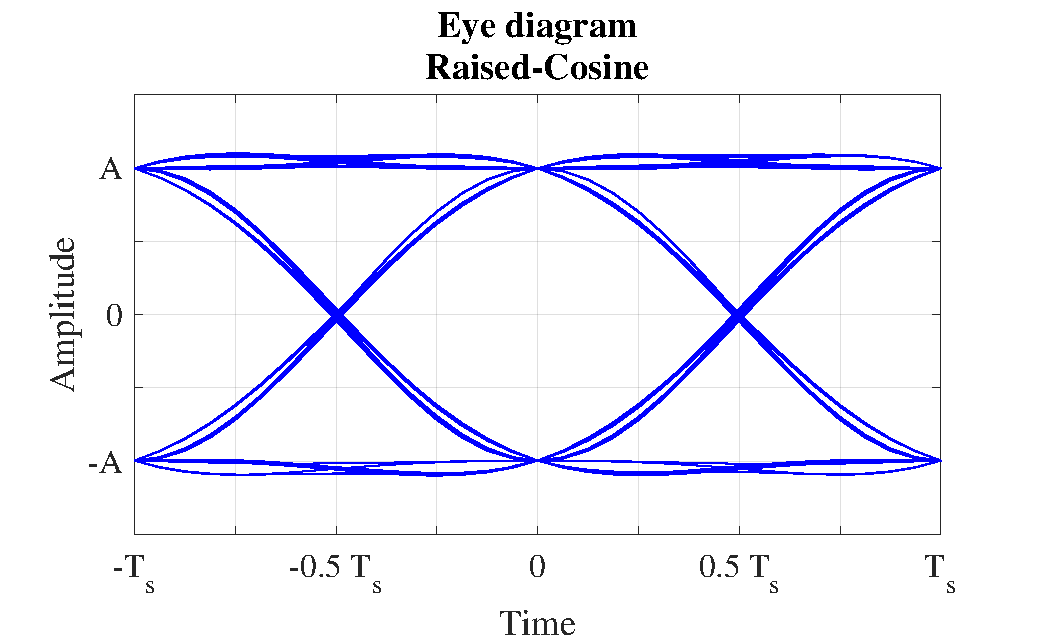
\includegraphics[width=\textwidth]{./sdf/m_qam_system/figures/eyes/ISI/RC.pdf}
		\end{minipage}
		\caption{Eye diagrams of two signals without noise: on the left,
			shaped with a single root-raised-cosine filter and affected by ISI; on the right,
		shaped using a raised-cosine filter, showing no signs of ISI.}
		\label{fig:ISIcomp}
	\end{figure}

%	\begin{figure}[H]
%		\centering
%		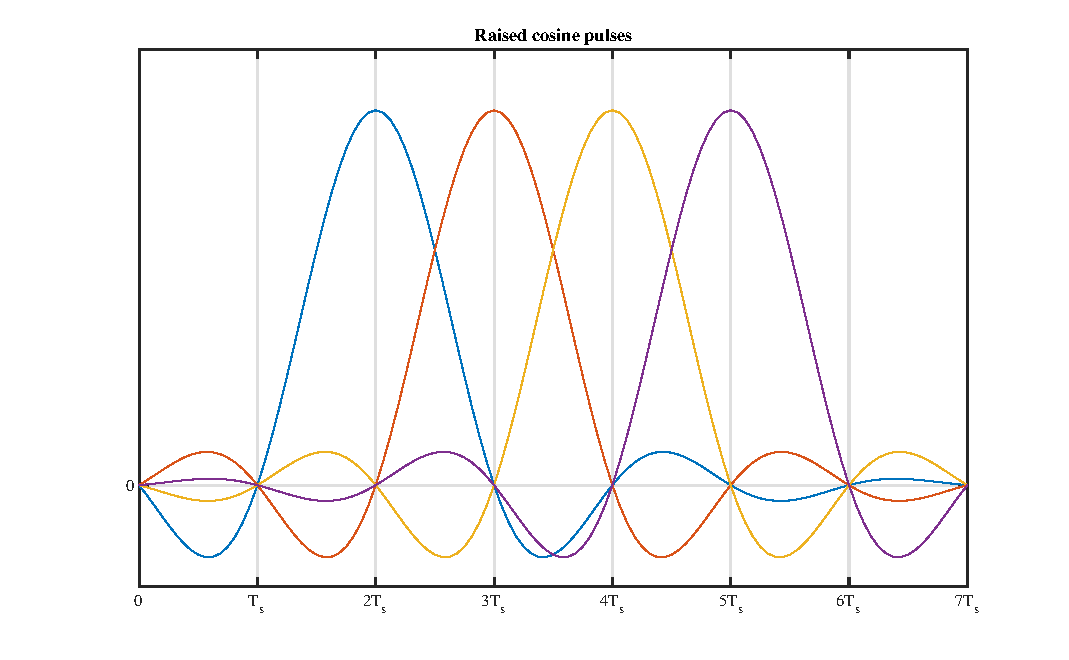
\includegraphics[width=\textwidth]{./sdf/m_qam_system/figures/eyes/ISI/pulsesRaisedCosine.pdf}
%		\caption{Sequence of four raised-cosine pulses. It can be seen that at $t=nT_s$,
%		every pulse equals zero except one, which will have its maximum value there.}
%		\label{fig:ISIcomp}
%	\end{figure}


	Optimal detection often requires the implementation of matched
	filters~\cite{schwartz90}. This is because in addition to avoiding ISI, it is
	desirable to maximize the SNR before sampling the signal, and in order to achieve
	both these objectives simultaneously, a matched filter should be used. This is
	done by
	implementing in the receiver a filter similar to the one used to initially
	shape the pulses. The pulse-shaping process becomes divided between the
	transmission and reception stages. Provided that an approppriate filter is
	chosen, the resulting signal can still be free of ISI, while reducing the
	noise power in the final sampled signal.

	The first filter, implemented on the transmitter, will convert the discrete
	symbols into continuous shapes, so that it can be transmitted on a modulated
	signal. The filter at the receiver finalizes the shaping process, making the
	signal reach the desired shape for symbol identification. In addition, it
	decreases the amount of noise affecting the signal.

	With matched filtering, the raised-cosine can be implemented by having the
	filters at the transmitter and receiver be root-raised-cosine filters.
	The end result will be signal with the same shape as if a raised cosine
	filter were used at the transmitter.

	The root-raised-cosine is defined as a filter for which the square of the
	frequency response is equal to the frequency response of the raised cosine
	filter. Its time domain impulse response
	given by\cite{nguyen09}:

	\begin{equation}\label{eq:rrcTD}
		h_{RRC}(t) = \frac{(4\beta t/T_s)\cos\big[\pi(1+\beta)t/T_s\big] +
		\sin\big[\pi(1-\beta)t/T_s\big]}
		{(\pi t/T_s)\big[1-(4 \beta t/T_s)^2\big]}
	\end{equation}

%	Having a signal pass through the same root-raised-cosine filter twice is equivalent
%	has having it pass a raised-cosine filter.

	\subsubsection{Noise}
	So far we have neglected to include any source of noise in this analysis.
	Several possible noise sources can be considered, either in the optical
	or in the electrical part of the system. As shown in
	Figure~\ref{fig:rxDiagram}, for now we will only consider the existence of
	optical noise,  and we will consider that the noise added is ASE which could
	originate from a EDFA. The ASE field can be represented as a sum of terms as
	follows ~\cite{crognale14, olsson89}:

	\begin{align}
		E_{\text{ASE}x} &= \sum_{k=-B_\nu}^{B_\nu} \sqrt{2 n_{0o} \delta \nu}
		\cos{((-\omega + 2\pi k \delta \nu) t + \phi_{kx})} \\
		E_{\text{ASE}y} &= \sum_{k=-B_\nu}^{B_\nu} \sqrt{2 n_{0o} \delta \nu}
		\sin{((-\omega + 2\pi k \delta \nu) t + \phi_{ky})}
	\end{align}

	\noindent where $B_\nu = B_{\text{opt}}/(2 \delta \nu)$, $B_{\text{opt}}$ is the optical
	bandwidth and $\delta \nu$ is small frequency interval. We can write an
	expression for the optical noise spectral density $n_{0o}$ considering the use of a number
	$N_A$ of cascaded EDFA's. Assuming that all amplifiers are similar and equally
	spaced, and that the gain in each EDFA is just enough to compensate the fiber
	losses in the distance between them, we have~\cite{agrawal12}:

	\begin{equation}
		n_{0o} = N_A n_{\text{sp}} (G_o-1) h\nu
	\end{equation}

	Here, $n_{\text{sp}}$ is the EDFA's spontaneous emission factor, $h\nu$ is the
	photon energy.
	In additon, $\phi_{kx}$ and $\phi_{ky}$ are independent uniform random
	variables representing random phases for each of the terms in the summation,
	and $G_o$ is the amplifiers'  optical gain as defined in
	equation~\ref{fig:ampGain}.
	This field is added to equation~\ref{eq:sigEq}, giving rise to three noise
	terms from different interactions:

	\begin{itemize}
		\item ASE-LO, from the interaction with the local oscillator;
		\item ASE-SIG, from the interaction with the transmitted signal;
		\item ASE-ASE, from the interaction with itself.
	\end{itemize}

	For now, we will consider only the ASE-LO component, which  is close enough
	to additive white Gaussian noise. In addition, it is typically the strongest,
	as usually the LO power is much greater than either the signal or the ASE. The
	variance, or noise power, generated by this component at each pair of balanced
	photodiodes is given by~\cite{crognale14}:

%		\sigma_{\text{ASE}-\text{SIG}}^2 &= 2 \eta^2 \alpha P__s P_{\text{LO}} n_{0o} B_N \\
%		\sigma_{\text{ASE}-\text{ASE}}^2 &= \sqrt{2} \eta P_{\text{LO}} n_{0o} B_N \\
	\begin{equation}\label{eq:noiseComps}
		\sigma_{\text{ASE}-\text{LO}}^2 = 2 \eta^2 P_{\text{LO}} n_{0o} B_N =
		2 \eta^2 P_{\text{LO}} N_A n_{\text{sp}} (G_o - 1) h\nu B_N
	\end{equation}

	\noindent Here, $B_N$ is the electrical noise bandwidth. Notice that the total noise
	power is proportional to this bandwidth, so keeping it closer to the signal's
	bandwidth limits the total noise to a minimum. This noise is also amplified at
	the transimpedance amplifier, so we get a voltage variance equal to:

	\begin{equation}\label{eq:noiseCompsAmp}
		\sigma_{\text{ASE}-\text{LO}}^2 = 2 \eta^2 G_e^2 P_{\text{LO}} N_A n_{\text{sp}} (G_o - 1) h\nu B_N
	\end{equation}

	Considering the generated noise to be independent from the signal, let $x(t)$
	be the signal at the ADCs, sampled at a given instant $t$ for either the
	in-phase or quadrature component. $x(t)$ has two components:

	\begin{equation}\label{eq:sampledComponents}
		x(t) = s(t) + n(t)
	\end{equation}

	\noindent where the component $s(t)$ corresponds to the received signal, and
	$n(t)$ corresponds to the noise component. For $t = nT_s$, as mentioned in
	equations~\ref{eq:rxSymbolsi} and~\ref{eq:rxSymbolsq}, $s(t) = \pm A$. The
	noise component, being AWGN, has constant power spectral density, and follows
	a Gaussian distribution with zero mean and variance equal to the noise power
	as described in equation~\ref{eq:noiseCompsAmp}.

	It's possible to remove the exceeding noise through filtering. This is
	done by the matched filter, as mentioned in the previous
	section. The filter essentially decreases the bandwidth, removing all
	the noise at frequencies not contained in $f < \big|{1}/{(2T_s)}\big|$, while
	not causing intersymbol interference in the transmitted signal.

	Let us consider a signal as described in
	Equation~\ref{eq:sampledComponents}, with $ a(t) = A_p~p(t) $, where $A_p$ is the peak
	amplitude of the signal and $p(t)$ is the shape of the pulse. In addition, let $n(t)$ be AWGN
	of spectral density $G_n(f) = {n_0}/{2}$. Finally, assume that the filter
	at the receiver has a frequency response $H(f)$.
	The filter is similar to the shape of the pulse , but reversed in time and
	shifted by a time delay, such that it maximizes the SNR~\cite{carlson86}.
	The energy contained in the pulse that enters the receiver filter depends on the
	pulse amplitude and on its shape, and it is given by:
%
	\begin{eqnarray}\label{eq:pulseEnergy}
		E_p = \int_{-\infty}^{\infty} {|A(f)|}^2 df = A_p^2 \int_{-\infty}^{\infty} {|P(f)|}^2 df
	\end{eqnarray}

	The amplitude of the signal component after the receiver filter $H(f)$, at a
	given sampling time $t=t_0+t_d$, is:

	\begin{eqnarray}
		A = \mathfrak{F}^{-1}\left[H(f) A(f)\right]\big|_{t=t_0+t_d} = A_p \int_{-\infty}^{+\infty} H(f) P(f) e^{+j \omega t_d}df
	\end{eqnarray}

	Similarly, the noise power at the receiver filter output is given by:

	\begin{eqnarray}
		N_o = \int_{-\infty}^{+\infty} {|H(f)|}^2 G_n(f) df = \frac{n_0}{2} \int_{-\infty}^{+\infty} {|H(f)|}^2
	\end{eqnarray}

	This means that the peak signal power to mean noise power ratio at the filter
	output is given by:

	\begin{eqnarray}
		\frac{A^2}{N_o} &= A_p^2 \frac{\big|\int_{-\infty}^{+\infty} |H(f) P(f)e^{j\omega t_d} df\big|^2}{\int_{-\infty}^{+\infty} {|H(f)|}^2 G_n(f) df}\\\nonumber
											&= A_p^2 \frac{\big|\int_{-\infty}^{+\infty} |H(f) P(f)e^{j\omega t_d} df\big|^2}{\frac{n_0}{2}\int_{-\infty}^{+\infty} {|H(f)|}^2df}
	\end{eqnarray}

	It can be shown that a matched filter maximizes the ratio above, so that it
	becomes~\cite{carlson86} :

	\begin{equation}
		\frac{A^2}{N_o} = \frac{A_p^2}{n_0/2} \int_{-\infty}^{+\infty} |P(f)|^2 df = \frac{A_p^2}{n_0/2} \int_{-\infty}^{+\infty} p(t)^2 dt
	\end{equation}

%
%	This shows that the SNR and, therefore, the error probability after filtering is dependent on
%	the energy of each symbol and the noise spectral density. However, even though
%	the relation does not directly depend on the pulse shape, the energy of each
%	symbol still depends on the pulse shape. The energy of the symbol results from
%	an integration over the symbol period.


%	It can be
%	shown~\cite{carlson86} that, according to what has been shown so far

	Thus, substituting from equation~\ref{eq:pulseEnergy}, the following relation
	can be verified for the signal after the matched filter:

	\begin{equation}\label{eq:amp2en}
		\frac{A^2}{N_o} = \frac{2 E_b}{n_0}
	\end{equation}

	Here, $A$ is the amplitude of $s(t)$ at the output of the matched filter,
	$N_o$ is the corresponding noise power, $E_b$ is the energy per bit and $n_0/2$
	is the two-sided noise spectral density, obtained from
	equation~\ref{eq:noiseCompsAmp} from
	$n_0 = \sigma_{\text{ASE}-\text{LO}}^2 / B_N$.


	$x(t) = s(t) + n(t)$ remains a valid representation of the signal for each of
	the quadratures after the matched filter, even if $s(t)$ and $n(t)$ have
	changed. In addition, $n(t)$ remains additive Gaussian noise. Therefore,
	$x(t)$ after the matched filter, at time $t = nT_s$ is also a Gaussian random
	variable, and has mean $A^2$ and variance $N_o$. This relation will show
	itself useful during the analysis of the error probability in the following
	section.


	\subsubsection{Bit error rate}
	For each quadrature, an error occurs in one of two situations: when a 0 is
	transmitted but a 1 is identified, or a 1 is transmitted and a 0 is
	identified.

	As previously mentioned, the values sampled at sampling time $t = nT_s$, which are used to
	identify the received symbols, follow a Gaussian
	distribution. Using the constellation from
	Figure~\ref{fig:const_2m}, with a decision boundary halfway between $A$ and
	$-A$, an error occurs in two situations:

	\begin{equation}
		\begin{cases}
			x(t) < 0, \quad \text{if } s(t)=A \\
			x(t) > 0, \quad \text{if } s(t)=-A
		\end{cases}
		\implies \quad
		\begin{cases}
			n(t) < -A, \quad \text{if } s(t)=A \\
			n(t) > A, \quad \text{if } s(t)=-A
		\end{cases}
	\end{equation}

	This is illustrated in Figure~\ref{fig:gauss},
	where the probability of error is shown by the colored area under the
	curves~\cite{schwartz90}.

	\begin{figure}[]
		\centering
		\begin{minipage}{1\textwidth}
			\centering
			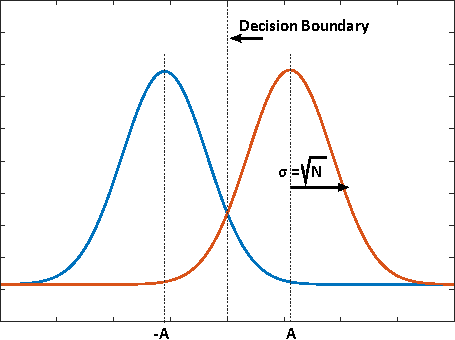
\includegraphics[width=0.50\textwidth]{./sdf/m_qam_system/figures/gaussians.pdf}
			\subcaption{}
		\end{minipage}
		\begin{minipage}{0.35\textwidth}
			\centering
			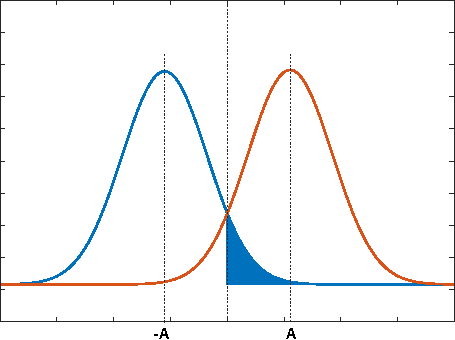
\includegraphics[width=1\textwidth]{./sdf/m_qam_system/figures/gaussian_error_blue.pdf}
			\subcaption{}
		\end{minipage}
		\begin{minipage}{0.35\textwidth}
			\centering
			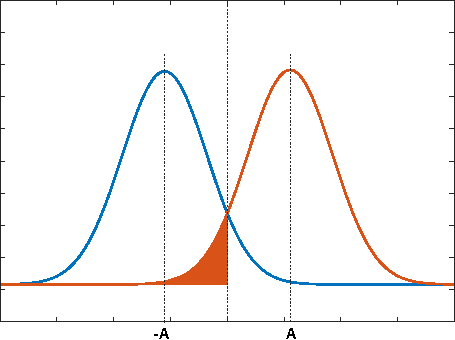
\includegraphics[width=1\textwidth]{./sdf/m_qam_system/figures/gaussian_error_orange.pdf}
			\subcaption{}
		\end{minipage}
		\caption{Probability density functions for $x(t) = s(t) + n(t)$, with
		$s(t)=\pm A$ at the time of sampling, and $n(t)$ as a Gaussian variable of
	zero mean and variance $N$. The colored areas below the curves on the right
represent the probability of error for each transmitted bit.}
		\label{fig:gauss}
	\end{figure}

	The probability of bit error (assuming equal emission probabilities for both bits) can be expressed as:

	\begin{equation}
		\begin{split}
			P_{be} &= P_0 P_{e0} + P_1 P_{e1} = \frac{1}{2} P_{e0} +
			\frac{1}{2} P_{e1} \\
						 &= \frac{1}{2} \Bigl[\Pr\Bigl(n(t)<-A\Bigr) +
						 \Pr\Bigl(n(t)>A\Bigr)\Bigr]
		\end{split}
	\end{equation}

	$P_0$ and $P_1$ are the probabilities of the transmitted bit being a 0 or
	1, respectively, and $P_{e0}$ and  $P_{e1}$ are the respective probabilities of
	error. It follows that the probability of bit error can be described using the
	Q-function, or alternatively, the complementary error function.

	\begin{equation}\label{eq:berMQAM}
		P_{be} =  Q\left({\frac{A}{\sqrt{N_o}}}\right) = \frac{1}{2}
		\text{erfc}\left({\frac{A}{\sqrt{2 N_o}}}\right)
	\end{equation}

	The probability of bit error is also known as bit error rate, or BER.

	We have worked on the probability of bit error for each
	quadrature independently. However, assuming a gray code, and knowing that the
	carriers are uncorrelated, an error in each carrier is independent from the
	other~\cite{nguyen09}. This can be verified by noting that the even bits are
	dependent only on one of the quadratures, and the odd bits depend on the
	other. Therefore, as half the bits are even and half are odd, and assuming
	that the constellation is symmetrical, it follows that the error rate is the
	same as for each quadrature independently.

	\begin{equation}
		\begin{split}
			\text{BER} &= P_{\text{odd}} P_{\text{oddError}} +
								 P_{\text{even}}P_{\text{evenError}}\\
								 &= \frac{1}{2} P_{\text{oddError}} + \frac{1}{2}
								 P_{\text{evenError}}\\
								 &= \frac{1}{2} \left(Q\left({\frac{A_{even}}{\sqrt{N_{even}}}}\right)
								 +Q\left({\frac{A_{odd}}{\sqrt{N_{odd}}}}\right) \right)\\
								 &= Q\left({\frac{A}{\sqrt{N_o}}}\right)
		\end{split}
	\end{equation}


	Looking back at equation~\ref{eq:amp2en}, we can also define the probability
	of error as a function of the energy per bit:

	\begin{equation}\label{eq:berMod}
		P_{be} =  Q\left(\sqrt{\frac{2 E_b}{{n_0}}}\right) = \frac{1}{2} \text{erfc}\left(\sqrt{\frac{E_b}{n_0}}\right)
	\end{equation}

	While the BER can be calculated by analyzing each quadrature independently,
	the probability of symbol error is different. In this case, a symbol error
	happens whether there is an error in one of the quadratures or in both. There
	is no distinction between these cases. Therefore, the calculation of the
	symbol error rate requires a different approach. Let us first define the
	probability of correctly identifying a symbol.

	\begin{equation}
		P_C = (1 - P_{be})^2
	\end{equation}

	From this, the probability of symbol error is:

	\begin{equation}
		\begin{split}
			P_{Se}  &= 1-P_C \\
							&= 1 - \left(1 - Q \left({\frac{A}{\sqrt{N_o}}}\right)\right)^2
			\\
							&= 2 Q\left({\frac{A}{\sqrt{N_o}}}\right)\left[1-\frac{1}{2} Q
			\left({\frac{A}{\sqrt{N_o}}}\right)\right] \\
							&= 2 Q\left({\sqrt{\frac{2E_b}{{n_0}}}}\right)\left[1-\frac{1}{2}
			Q \left({\sqrt{\frac{2E_b}{{n_0}}}}\right)\right]
		\end{split}
	\end{equation}

	\begin{figure}
		\centering
		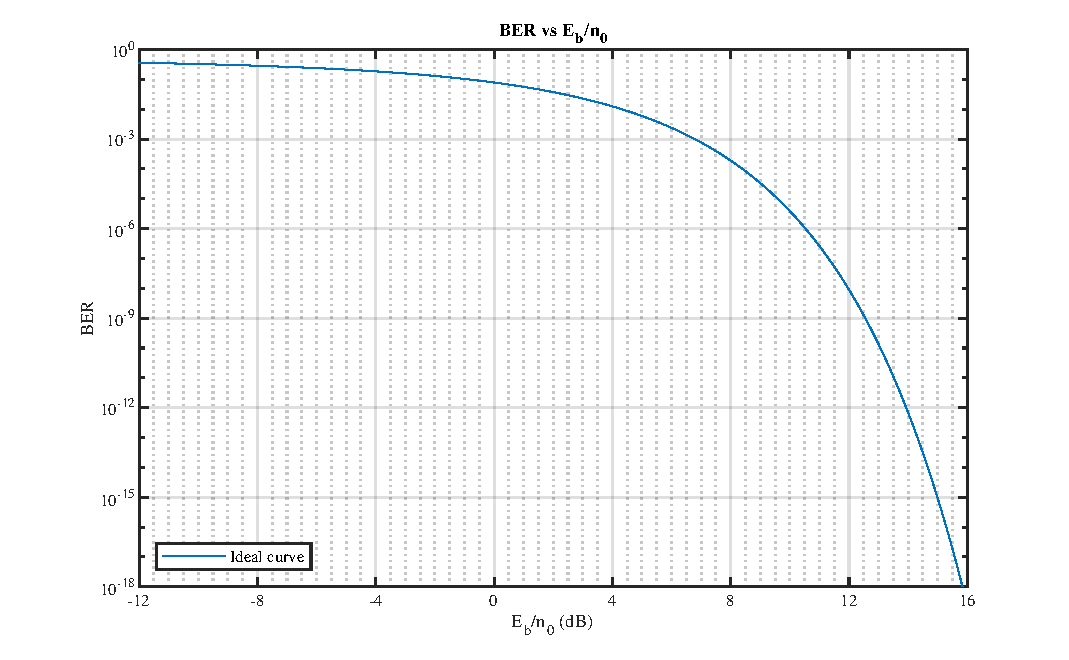
\includegraphics[
		width=1\textwidth]{./sdf/m_qam_system/figures/berPlots/ebn0Curve.pdf}
		\caption{QPSK theoretical BER curve as a function of the ratio of energy per
		bit and the noise spectral density in dB.\label{fig:QPSK_ebn0_curve}}
	\end{figure}

	It's worth noting that these equations are only valid for M=4, as in that case
	the system is similar to QPSK with a 4 point constellation. For $M > 4$ a
	different approach is required for calculating the BER, as the decision
	borders will be very different.

	We can now write the expected bit error rate as a function of the system
	parameters. To get $E_b$, we can start by picking up the equations for the
	signal waveforms which are sampled and measured at the ADC, described in
	Equations~\ref{eq:photocurrentI} and~\ref{eq:photocurrentQ}.

	\begin{equation}
		E_b(t) = G_e^2 \eta^2 {G_o P_s P_{lo}} \frac{T_s}{2} \label{eq:energyPerBit}
		%E_b(t) = G_e^2 \eta^2 {G_o P_s P_{lo}} \sin^2{(\phi_{s}(t))} \frac{T_s}{2} \label{eq:photocurrentQ}
	\end{equation}

	To get $n_0$, we start with equation~\ref{eq:noiseCompsAmp}, which gives the
	noise variance at the ADC's. The noise power spectral density will be the
	ration of this variance to the electrical bandwidth of the receiver. So we
	get:

	\begin{equation}\label{eq:sampledn0}
		\begin{split}
			n_0 &= \frac{2 \eta^2 G_e^2 P_{\text{LO}} N_A n_{\text{sp}} (G_o -
			1)h\nu B_N}{B_N} \\
					&= 2 \eta^2 G_e^2 P_{\text{LO}} N_A n_{\text{sp}} (G_o - 1) h\nu \\
					&= 2 \eta^2 G_e^2 P_{\text{LO}} n_{0o}
		\end{split}
	\end{equation}

\pagebreak